% ======================================================================
\section{Worked examples}
\label{sec:results}
% ======================================================================

The figures of this section are produced by the notebooks (\code{notebooks/01}--\code{05}) with the parameters of
\cref{sec:numerics}; the numbers quoted are printed by the notebooks.

\subsection{Electrostatics of the junction (notebook 01)}

\begin{figure}[htbp]
\centering
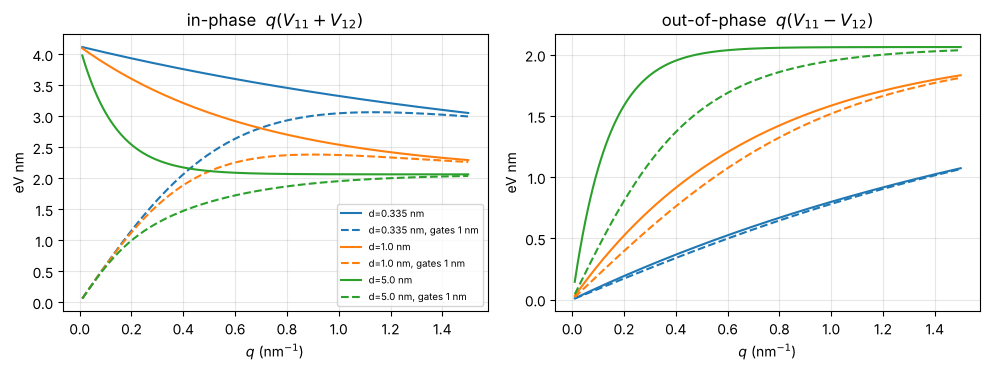
\includegraphics[width=0.92\textwidth]{figures/fig_coulomb_channels.png}
\caption{In-phase and out-of-phase Coulomb channels $q(V_{11}\pm V_{12})$ of two sheets in hBN
($\varepsilon_\parallel=6.41$, $\varepsilon_z=3$) for three separations, without (solid) and with (dashed) gates 1 nm
away. Without gates $qV_+\to4\pi e^2/\bar\varepsilon=4.13$ eV\,nm at $q\to0$ and both tend to $2\pi e^2/\bar\varepsilon$ at
$q\gg1/d$; the out-of-phase channel vanishes linearly, $qV_-\simeq2\pi e^2qd/\varepsilon_z$. Gates kill the long-range
in-phase part and barely touch the out-of-phase one.}
\label{fig:channels}
\end{figure}

The closed forms of \cref{sec:electrostatics} are reproduced to machine precision (e.g.\ $V_{12}/V_{11}=e^{-\kappa d}=0.8634$
at $d=0.335$ nm), the dispersive hBN kernel is passive in the Reststrahlen bands, and the capped-slab kernel
interpolates between its limits (\cref{fig:channels}).

\subsection{Doped monolayer graphene (notebook 02)}

The SLG$|$1 nm hBN$|$SLG junction with $n=10^{12}$ cm$^{-2}$ in both sheets ($k_F=0.177$ nm$^{-1}$, $E_F=116.6$ meV,
$\bar\varepsilon=4.39$, graphene fine-structure constant $e^2/\bar\varepsilon\hbar v_F=0.50$). The closed-form $\chi^0$ agrees with
a brute-force Lindhard sum to $<6\times10^{-3}D(E_F)$.

\begin{figure}[htbp]
\centering
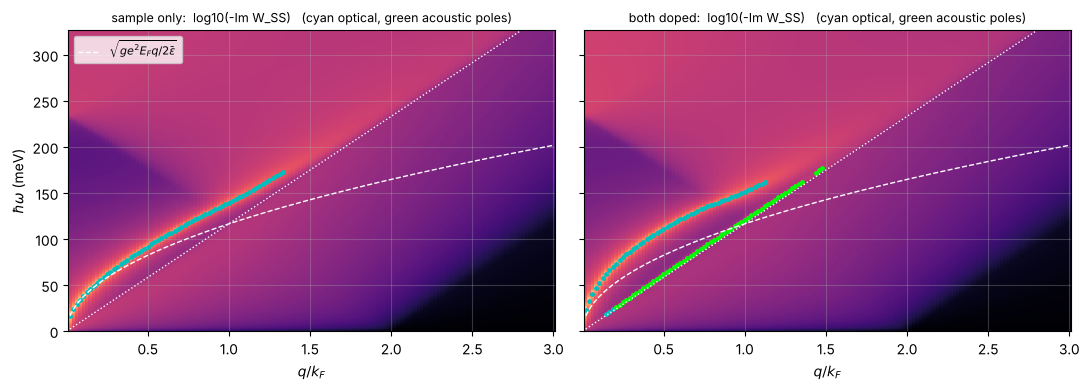
\includegraphics[width=\textwidth]{figures/fig_slg_plasmons.png}
\caption{Loss $\log_{10}(-\Imm W_{SS})$ of the sample sheet with the plasmon poles found as minima of
$|\lambda_{\min}(\varepsilon)|$. Left: inert tip, one optical branch following $\sqrt{ge^2E_Fq/2\bar\varepsilon}$ (dashed) at small
$q$. Right: both sheets doped, an additional acoustic branch (green) with $v_{\rm ac}/v_F=1.048$, above the
intraband continuum edge $\omega=v_Fq$ (dotted) as it must be. Both branches enter the continuum and stop being
poles; at 53\% of the $q$ points there is no pole at all.}
\label{fig:slgplasmons}
\end{figure}

\begin{figure}[htbp]
\centering
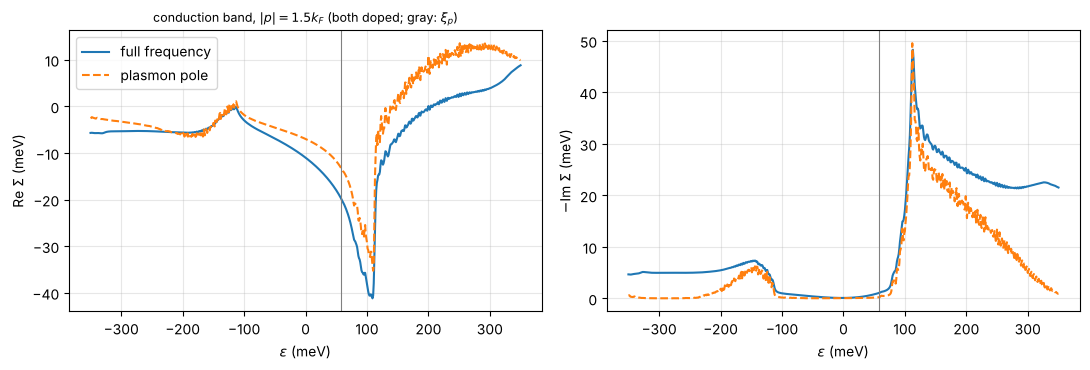
\includegraphics[width=\textwidth]{figures/fig_slg_sigma.png}
\caption{$\Sigma$ of the conduction band at $|\bp|=1.5k_F$ (bare energy $\xi_{\bp}=58$ meV, gray). Full frequency (solid)
vs plasmon-pole approximation (dashed). The PPA reproduces the plasmon-emission threshold at $\eps\simeq110$ meV but
misses the continuum contribution to $-\Imm\Sigma$ at high energy and the associated part of $\Ree\Sigma$; its ripples
come from the discrete set of poles $(\bq,\omega_n(\bq))$ on the $q$ grid.}
\label{fig:slgsigma}
\end{figure}

\begin{figure}[htbp]
\centering
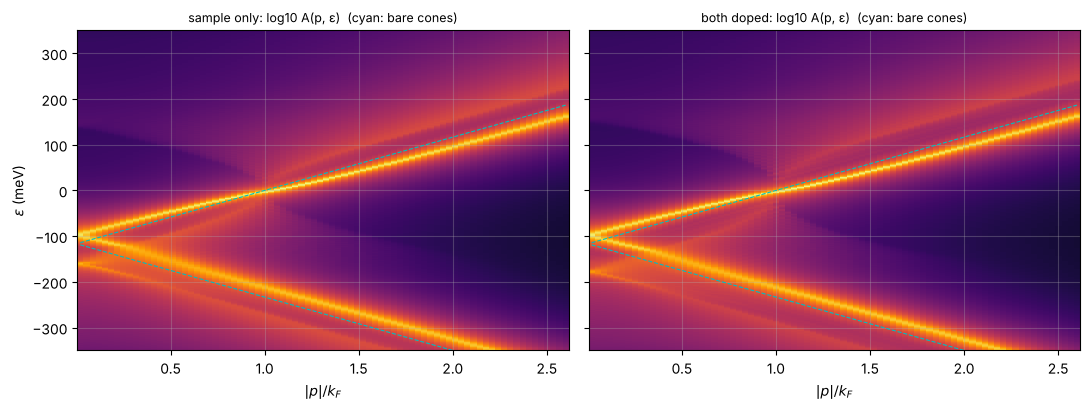
\includegraphics[width=\textwidth]{figures/fig_slg_spectral.png}
\caption{$\log_{10}A(|\bp|,\eps)$ of the sample, inert tip (left) and doped tip (right); cyan: bare cones. The
quasiparticle bands are flattened by the correlation self-energy ($v^*/v_F=0.92$, $Z\simeq0.82$--$0.83$); the faint
replica bands displaced away from $E_F$ are the plasmaron satellites, the strongest one below the Dirac point at
small $|\bp|$. At $|\bp|=1.33k_F$ the window $\pm350$ meV holds 98.8\% of the spectral weight.}
\label{fig:slgspectral}
\end{figure}

\begin{figure}[htbp]
\centering
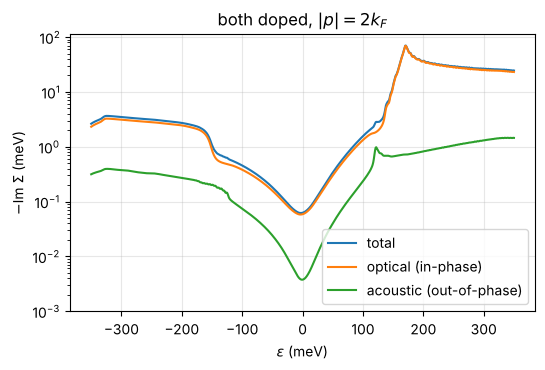
\includegraphics[width=0.55\textwidth]{figures/fig_slg_channels.png}
\caption{Layer-channel decomposition (\cref{eq:channels}) of $-\Imm\Sigma$ at $|\bp|=2k_F$, both sheets doped. The split
is exact (additivity $10^{-15}$); the acoustic (out-of-phase) channel carries $\simeq4\%$ of $\|\Sigma\|$.}
\label{fig:slgchannels}
\end{figure}

The kernel route reproduces the direct frequency integration to $1.3\times10^{-4}$ (1.1 s against 78 s per
$\bk$). The plasmaron satellites of \cref{fig:slgspectral} are the features probed by the QTM in
\cref{sec:resqtmslg}; the acoustic plasmon of the junction contributes little to the sample self-energy at a 1 nm
spacing because its weight in $W_{SS}$ is small: the out-of-phase Coulomb channel $V_-\propto d$ is weak
(\cref{sec:channelsV,fig:slgchannels}).

\subsection{Twisted bilayer graphene (notebook 03)}

\begin{figure}[htbp]
\centering
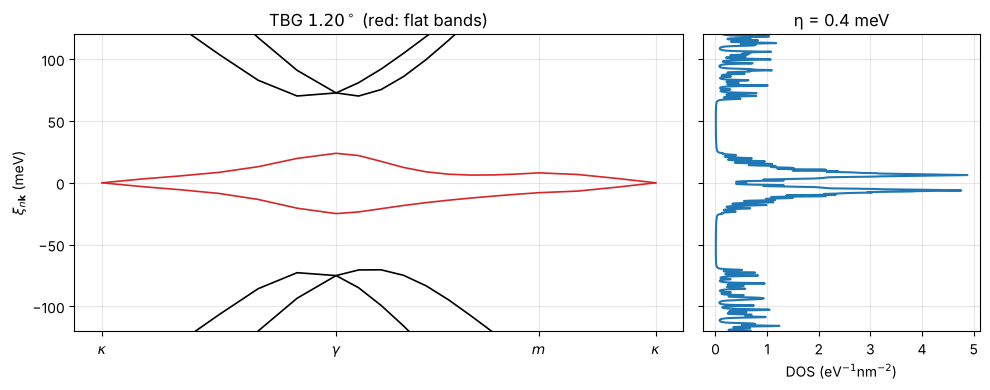
\includegraphics[width=0.9\textwidth]{figures/fig_tbg_bands.png}
\caption{Continuum bands of TBG at $1.20^\circ$ ($u_{AB}=117$ meV, $u_{AA}=0.7u_{AB}$) along $\kappa$--$\gamma$--$m$--$\kappa$ of the
$18\times18$ mesh, and density of states. Flat bands (red): widths $24.9$ and $23.9$ meV, gaps of $44$ and $45.5$ meV to
the remote bands, chemical potential $\mu=+1.8$ meV at neutrality.}
\label{fig:tbgbands}
\end{figure}

\begin{figure}[htbp]
\centering
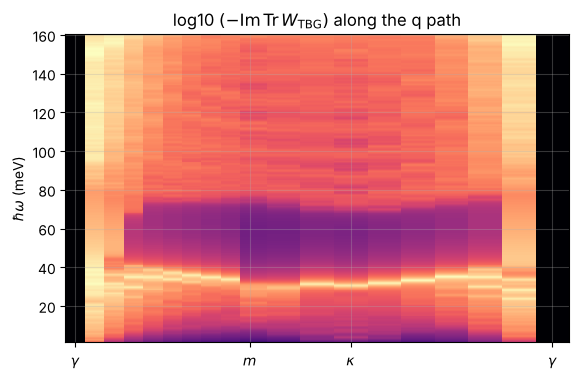
\includegraphics[width=0.62\textwidth]{figures/fig_tbg_loss.png}
\caption{Loss function $\log_{10}(-\Imm\Tr W_{\rm TBG})$ of the two TBG sheets in the SLG\,$|$\,1 nm hBN\,$|$\,TBG stack
(neutral tip), along $\gamma$--$m$--$\kappa$--$\gamma$ ($\bq=0$ is excluded, black), with the valley-summed $\chi^0$ of
\cref{eq:valleysym}. The nearly flat branch at $30$--$40$ meV is the flat-band plasmon, which lies in the gap between the intra-flat-band and
the flat-to-remote particle--hole continua~\cite{Wei2025}.}
\label{fig:tbgloss}
\end{figure}

\begin{figure}[htbp]
\centering
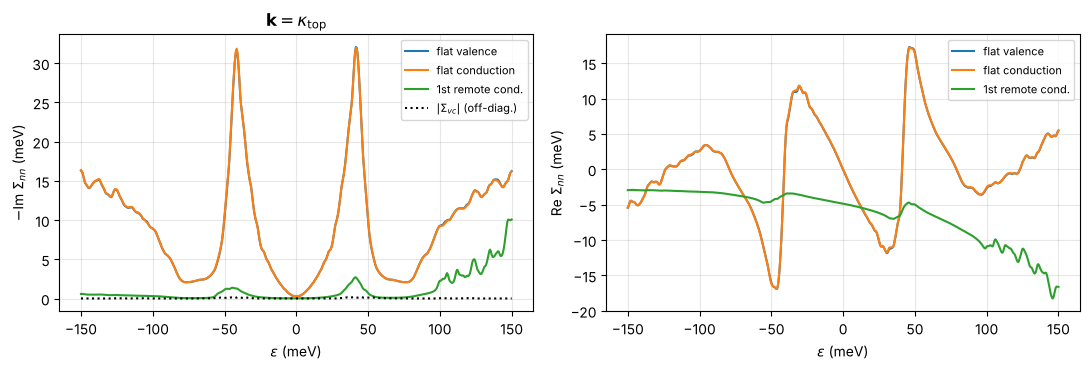
\includegraphics[width=\textwidth]{figures/fig_tbg_sigma.png}
\caption{Band-matrix G$_0$W self-energy at $\bk=\kappa_{\rm top}$ (diagonal elements; dotted: an off-diagonal element
between the two flat bands, which are degenerate at $\kappa$). The peaks of $-\Imm\Sigma$ of the flat bands at
$\eps\simeq\pm42$ meV are plasmon emission, $\eps\simeq\xi_{\rm flat}\pm\omega_{\rm pl}$; $\Ree\Sigma$ follows by
Kramers--Kronig. Kernel and direct contraction agree to $7\times10^{-5}$; $\Sigma$ is passive.}
\label{fig:tbgsigma}
\end{figure}

\begin{figure}[htbp]
\centering
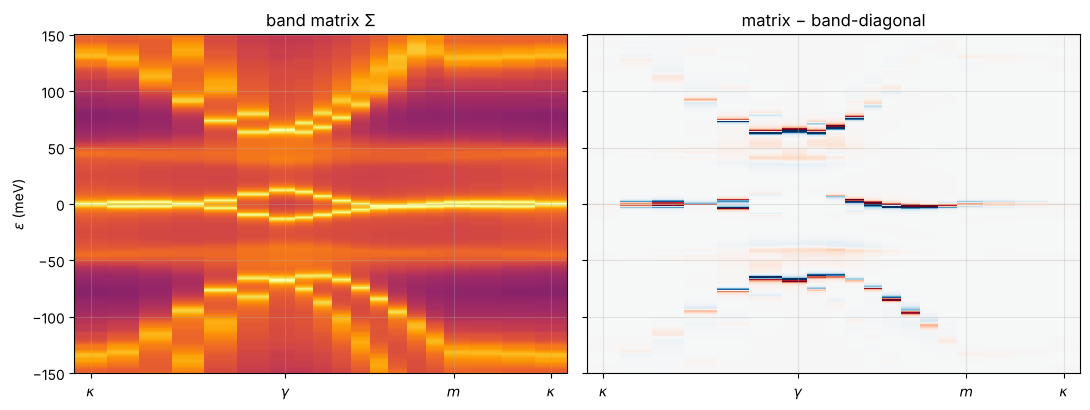
\includegraphics[width=\textwidth]{figures/fig_tbg_spectral.png}
\caption{Left: $\log_{10}\Tr A(\bk,\eps)$ from the matrix Dyson equation ($\eta_{\rm qp}=1$ meV) along
$\kappa$--$\gamma$--$m$--$\kappa$. Bright lines: quasiparticle bands; the faint, nearly $\bk$-independent lines at
$\simeq\pm(40$--$50)$ meV are the plasmon satellites of the flat bands. Right: difference between the band-matrix and the
band-diagonal $\Tr A$; it is concentrated where bands are close (flat bands, remote bands near $\gamma$).}
\label{fig:tbgspectral}
\end{figure}

\Cref{fig:tbgbands,fig:tbgloss,fig:tbgsigma,fig:tbgspectral} show the full chain for TBG. Two features deserve
comment. (i) The satellites of the flat bands are dispersionless because both the flat-band plasmon and the
intermediate flat-band states are nearly dispersionless; they are the structure the QTM is designed to detect
(\cref{sec:qtmtbg}). (ii) The band-off-diagonal self-energy changes the spectral function only where bands lie
within $|\Sigma|$ of each other, but there the change is of order one; the band-diagonal approximation is
therefore unreliable inside the flat-band manifold and at band crossings.

\subsection{QTM on doped graphene (notebook 04)}
\label{sec:resqtmslg}

\begin{figure}[htbp]
\centering
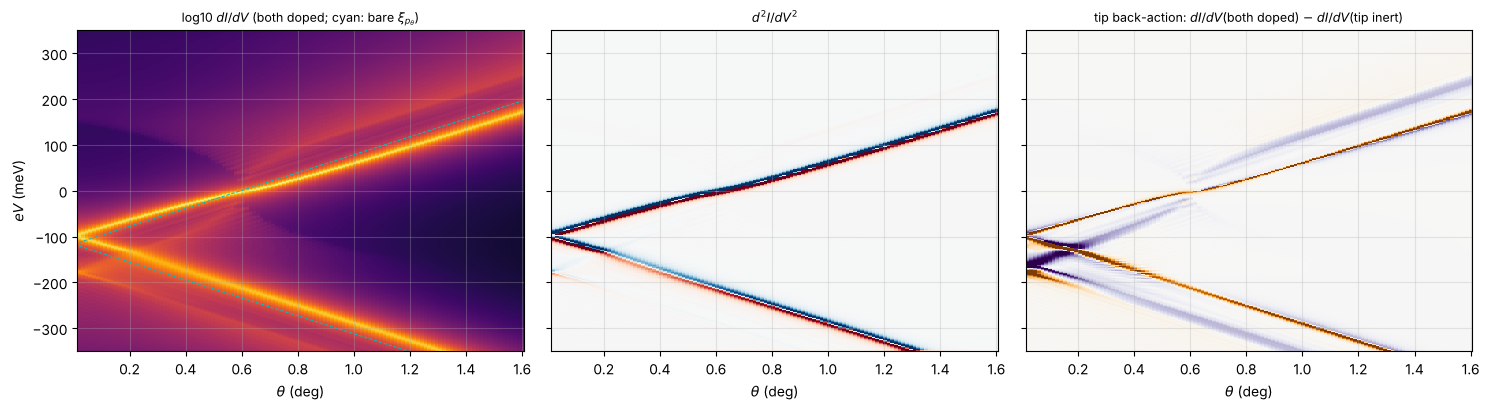
\includegraphics[width=\textwidth]{figures/fig_qtm_slg_map.png}
\caption{SLG tip\,$|$\,1 nm hBN\,$|$\,SLG sample, both at $10^{12}$ cm$^{-2}$. Left: $\log_{10}dI/dV$ from \cref{eq:didvslg}
(cyan: bare bands $\xi_{\pm}(\bp_\theta)$). Middle: $d^2I/dV^2$ after 1.5 meV Gaussian smoothing. Right: tip back-action,
the difference between a doped and an inert (non-screening) tip.}
\label{fig:qtmslgmap}
\end{figure}

\begin{figure}[htbp]
\centering
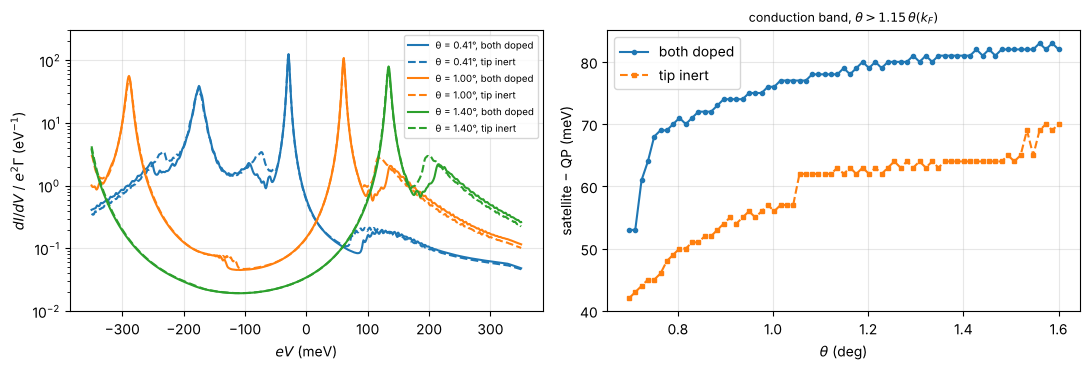
\includegraphics[width=\textwidth]{figures/fig_qtm_slg_cuts.png}
\caption{Left: line cuts of $dI/dV$ at three twist angles, doped (solid) and inert (dashed) tip. Right: offset of the
plasmaron satellite from the quasiparticle peak of the conduction band for $\theta>1.15\,\theta(k_F)$; it saturates
at $\simeq80$ meV with a doped tip and $\simeq63$ meV with an inert one.}
\label{fig:qtmslgcuts}
\end{figure}

The twist $\theta(k_F)=0.60^\circ$ brings the probed momentum to the Fermi surface, where the conduction-band ridge
crosses $eV=0$ (\cref{fig:qtmslgmap}); for $\theta\to0$ both ridges meet at the Dirac point, at $eV\simeq-100$ meV instead of $-E_F=-117$ meV because of
$\Ree\Sigma$. The chiral
matrix element changes the map by less than 0.7\% with respect to a constant one, as expected from
\cref{eq:didvslg}. The satellites run parallel to the quasiparticle ridges on the side away from $E_F$. Their
offset from the quasiparticle peak grows with $\theta$ and saturates (\cref{fig:qtmslgcuts}); doping the tip adds
its Drude weight to the in-phase plasmon of the junction and raises the offset by $\simeq17$ meV, the back-action
that a QTM with a metallic tip necessarily has. The offset is not the plasmon energy at a single momentum;
its origin and size are explained in \cref{sec:edge}.

\subsection{QTM on twisted bilayer graphene (notebook 05)}
\label{sec:resqtmtbg}

\begin{figure}[htbp]
\centering
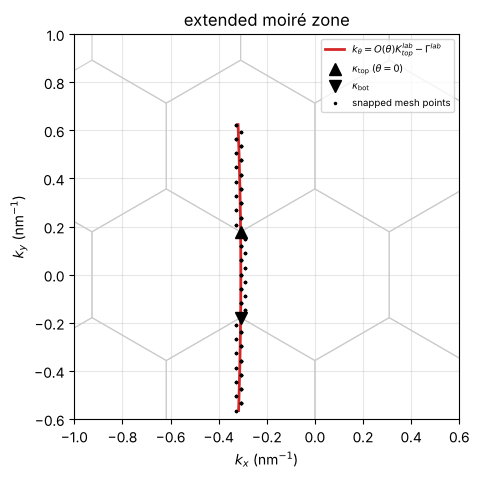
\includegraphics[width=0.48\textwidth]{figures/fig_qtm_tbg_trajectory.png}\hfill
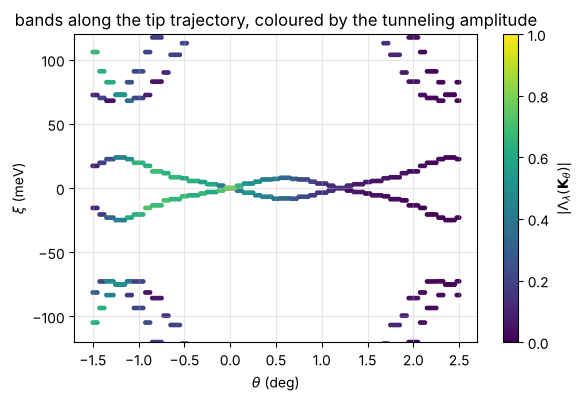
\includegraphics[width=0.5\textwidth]{figures/fig_qtm_tbg_bands.png}
\caption{Left: tip trajectory $\bk_\theta$, $\theta\in[-1.5^\circ,2.5^\circ]$, in the extended moir\'e zone (red), with the mesh
points it is snapped to. Right: the eight bands at
the snapped momenta, coloured by $|\Lambda_\lambda(\bk_\theta)|$ of \cref{eq:Lambdatbg}: near $\theta=0$ the tip sees the
flat bands through their top-layer Dirac-cone component; away from $\kappa_{\rm top}$ the weight moves out of the
computed band window.}
\label{fig:qtmtbgtraj}
\end{figure}

\begin{figure}[htbp]
\centering
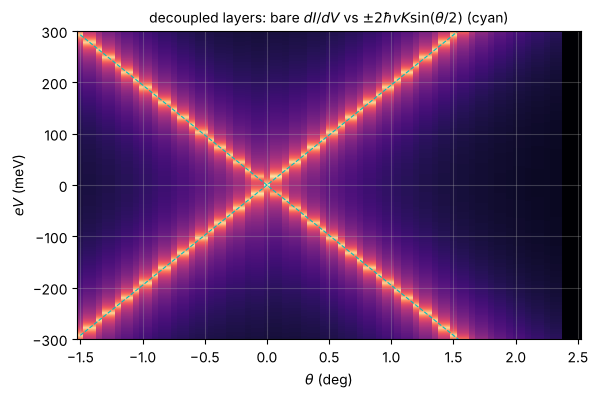
\includegraphics[width=0.62\textwidth]{figures/fig_qtm_tbg_decoupled.png}
\caption{Validation with the interlayer hopping switched off ($24\times24$ mesh, 16 bands): the bare conductance follows the
top-layer Dirac cone $eV=\pm2\hbar vK\sin(\theta/2)$ (cyan) for all $\theta$, also outside the first moir\'e zone,
because the amplitude is taken from the plane wave that unfolds the momentum (\cref{eq:Lambdatbg}). The map is dark
for $\theta\gtrsim2.4^\circ$, where $\bk_\theta$ leaves the plane-wave cutoff.}
\label{fig:qtmtbgdec}
\end{figure}

\begin{figure}[htbp]
\centering
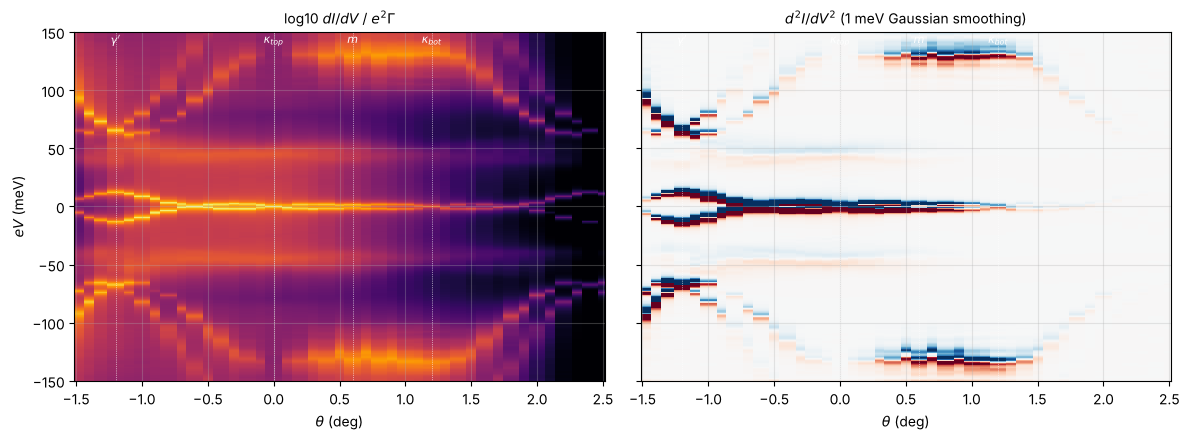
\includegraphics[width=\textwidth]{figures/fig_qtm_tbg_map.png}
\caption{$dI/dV(V,\theta)$ (left, log scale) and $d^2I/dV^2$ (right, 1 meV smoothing) of the SLG tip\,$|$\,1 nm hBN\,$|$\,TBG
junction at neutrality, from the band-matrix G$_0$W spectral function. Dotted lines: $\theta$ at which the tip probes
$\gamma'$, $\kappa_{\rm top}$, $m$ and $\kappa_{\rm bot}$. The map is piecewise constant in $\theta$ because the momentum is
snapped to the $18\times18$ mesh (36 distinct points).}
\label{fig:qtmtbgmap}
\end{figure}

\begin{figure}[htbp]
\centering
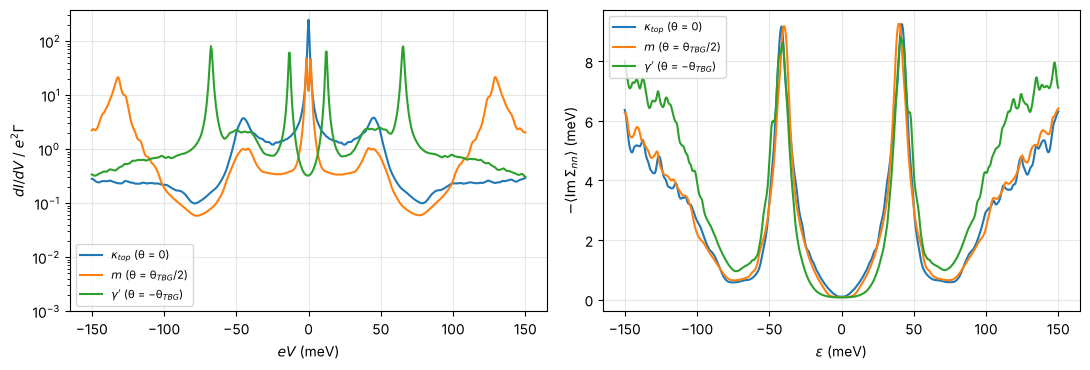
\includegraphics[width=\textwidth]{figures/fig_qtm_tbg_cuts.png}
\caption{Left: $dI/dV$ at $\kappa_{\rm top}$, $m$ and $\gamma'$. Right: band-averaged $-\Imm\Sigma_{nn}$ at the same momenta.
The quasiparticle peaks move with $\theta$; the satellites at $|eV|\simeq45$ meV do not, because they come from the
emission of the nearly dispersionless flat-band plasmon by flat-band electrons (the peaks of $-\Imm\Sigma$ at
$\pm40$ meV).}
\label{fig:qtmtbgcuts}
\end{figure}

\begin{figure}[htbp]
\centering
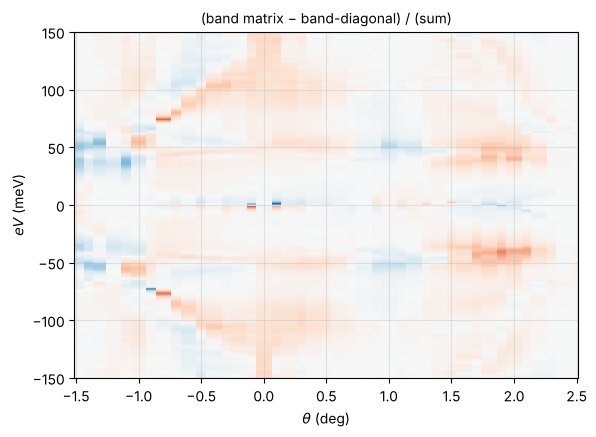
\includegraphics[width=0.62\textwidth]{figures/fig_qtm_tbg_interband.png}
\caption{Relative difference between the conductance from the band-matrix spectral function and from the
band-diagonal approximation, $(dI/dV_{\rm matrix}-dI/dV_{\rm diag})/(\text{sum})$, along the trajectory.}
\label{fig:qtmtbginterband}
\end{figure}

The physical kinematics puts the Dirac points of the two layers at $\theta=0$ and $\theta=\theta_{\rm TBG}$, where the
flat-band quasiparticle peak crosses $eV=0$, and the $\gamma$ point of the next zone at $\theta=-\theta_{\rm TBG}$, where the
flat bands are split by $\simeq25$ meV and the remote bands are visible at $\pm66$ meV
(\cref{fig:qtmtbgmap,fig:qtmtbgcuts}). The flat-band satellites appear as two horizontal stripes at
$|eV|\simeq45$ meV across the whole map; in $d^2I/dV^2$ they are weak compared with the quasiparticle edges. Beyond
$\theta\simeq1.8^\circ$ the map darkens because the top-layer weight at $\bk_\theta$ is carried by bands outside the
eight computed ones. The band-off-diagonal self-energy changes the conductance by $\simeq10\%$ in $L^2$ norm, locally
by tens of percent where bands are close (\cref{fig:qtmtbginterband}).
